%----------------------------------------------------------------------------------------
%    PACKAGES AND THEMES
%----------------------------------------------------------------------------------------

\documentclass[aspectratio=169,xcolor=dvipsnames]{beamer}
\usetheme{SimplePlus}
\usepackage{subcaption}
\usepackage{hyperref}
\hypersetup{colorlinks=true,linkcolor=.,urlcolor=blue,citecolor=blue}
\usepackage{amsmath}
\usepackage{xcolor}
\usepackage{graphicx}
\usepackage{booktabs}
\usepackage{tikz}
\usepackage{fontawesome5}

%----------------------------------------------------------------------------------------
%    TITLE PAGE
%----------------------------------------------------------------------------------------

\title{Explainable Disease Progression and Counterfactual Video Generation}
\subtitle{State of the Art \& Research Plan}

\author{Mohamed BOUFAFA }

\institute
{
    Mitacs Globalink Research Internship 2026 \\[0.3em]
    TÉLUQ University, Montreal, Canada \\[0.5em]
    \textbf{Supervisors:} \\
    Dr. Belkacem Chikhaoui (TÉLUQ) \\
    Dr. Belkacem Khaldi (Algeria)
}
\date{April 2026 -- August 2026}

%----------------------------------------------------------------------------------------
%    PRESENTATION SLIDES
%----------------------------------------------------------------------------------------

\begin{document}

% ============================================================================
% SLIDE 1: Title
% ============================================================================
\begin{frame}
    \titlepage
\end{frame}

% ============================================================================
% SLIDE 2: Presentation Roadmap
% ============================================================================
\begin{frame}{Presentation Roadmap}
    \begin{columns}[t]
        \begin{column}{0.48\textwidth}
            \begin{block}{\textbf{Part I: The Vision}}
                \begin{itemize}
                    \item Problem statement
                    \item Research objectives
                    \item Novel contribution
                \end{itemize}
            \end{block}
            
            \vspace{0.3em}
            
            \begin{block}{\textbf{Part II: State of the Art}}
                \begin{itemize}
                    \item Vision Transformers for Medical Imaging
                    \item Medical Vision-Language Models
                    \item Generative Models for Videos
                \end{itemize}
            \end{block}
        \end{column}
        
        \begin{column}{0.48\textwidth}
            \begin{block}{\textbf{Part III: Our Approach}}
                \begin{itemize}
                    \item Proposed pipeline architecture
                    \item Key components \& integration
                    \item Available resources \& models
                \end{itemize}
            \end{block}
            
            \vspace{0.3em}
            
        \end{column}
    \end{columns}
\end{frame}

% ============================================================================
% TRANSITION: PART I - THE VISION
% ============================================================================
\begin{frame}[plain]
    \centering
    \vfill
    \begin{beamercolorbox}[center,shadow=true,rounded=true]{title}
        \usebeamerfont{title}
        \textbf{Part I: The Vision}\\
        \vspace{0.5em}
        \large Problem $\to$ Objectives $\to$ Novel Contribution
    \end{beamercolorbox}
    \vfill
\end{frame}

% ============================================================================
% SLIDE 3: The Problem
% ============================================================================
\begin{frame}{The Problem: Medical AI Black Boxes}
    \begin{columns}
        \begin{column}{0.5\textwidth}
            \begin{block}{Current AI in Medical Imaging}
                \begin{itemize}
                    \item AI can \textbf{segment tumors} with high accuracy
                    \item Dice scores $\approx$ 0.85--0.90 on BraTS
                    \item AI can \textbf{generate synthetic images}
                    \item AI can produce \textbf{text reports}
                \end{itemize}
            \end{block}
            
            \vspace{0.5em}
            
            \begin{alertblock}{The Critical Gap}
                \textbf{No existing system:}
                \begin{itemize}
                    \item Explains \textit{why} in plain language
                    \item Shows \textit{what happens next} (progression)
                    \item Enables \textit{``what-if''} counterfactual scenarios
                \end{itemize}
            \end{alertblock}
        \end{column}
        
        \begin{column}{0.5\textwidth}
            \begin{block}{What Doctors Need}
                \begin{itemize}
                    \item Not just ``tumor'' or ``no tumor''
                    \item \textbf{Transparent reasoning}
                    \item ``The AI sees a mass in the cerebellum that grew since last scan''
                    \item \textbf{Future visualization}
                    \item How will this tumor progress?
                    \item What if we apply treatment X?
                \end{itemize}
            \end{block}
            
            \vspace{0.5em}
            
            \begin{exampleblock}{Our Goal}
                Build an AI that \textbf{sees}, \textbf{explains}, and \textbf{imagines the future}
            \end{exampleblock}
        \end{column}
    \end{columns}
\end{frame}

% ============================================================================
% SLIDE 4: Research Objectives
% ============================================================================
\begin{frame}{Research Objectives}
    \begin{columns}
        \begin{column}{0.55\textwidth}
            \begin{block}{\faIcon{bullseye} Five Core Objectives}
                \begin{enumerate}
                    \item \textbf{Data Pipeline:} Collect \& preprocess multi-modal medical imaging datasets (BraTS, TCGA, LIDC-IDRI)
                    
                    \vspace{0.3em}
                    \item \textbf{ViT Representations:} Train Vision Transformers for robust image understanding \& segmentation
                    
                    \vspace{0.3em}
                    \item \textbf{LLM Integration:} Connect visual features to language models for explainable outputs
                    
                    \vspace{0.3em}
                    \item \textbf{Video Generation:} Develop counterfactual progression videos using diffusion models
                    
                    \vspace{0.3em}
                    \item \textbf{Evaluation:} Validate with clinical metrics \& expert assessment
                \end{enumerate}
            \end{block}
        \end{column}
        
        \begin{column}{0.42\textwidth}
            \begin{block}{\faIcon{question-circle} Research Questions}
                \begin{itemize}
                    \item Can we integrate ViT, LLM, and diffusion into one pipeline?
                    \item Will explanations be medically accurate?
                    \item Can generated videos be clinically plausible?
                \end{itemize}
            \end{block}
            
            \vspace{0.5em}
            
            \begin{block}{\faIcon{lightbulb} Expected Impact}
                \begin{itemize}
                    \item Aid clinical decision-making
                    \item Enable patient communication
                    \item Support treatment planning
                \end{itemize}
            \end{block}
        \end{column}
    \end{columns}
\end{frame}

% ============================================================================
% TRANSITION: PART II - STATE OF THE ART
% ============================================================================
\begin{frame}[plain]
    \centering
    \vfill
    \begin{beamercolorbox}[center,shadow=true,rounded=true]{title}
        \usebeamerfont{title}
        \textbf{Part II: State of the Art}\\
        \vspace{0.5em}
        \large Vision Transformers $\to$ Vision-Language Models $\to$ Video Generation
    \end{beamercolorbox}
    \vfill
\end{frame}

% ============================================================================
% SLIDE 5: Vision Transformers - ViT Foundation
% ============================================================================
\begin{frame}{Vision Transformers: The Foundation}
    \begin{columns}
        \begin{column}{0.55\textwidth}
            \begin{block}{\href{https://arxiv.org/abs/2010.11929}{ViT}: An Image is Worth 16×16 Words}
                \small
                \textbf{Key Innovation (Dosovitskiy et al., 2021):}
                \begin{itemize}\setlength{\itemsep}{1pt}
                    \item Split image into 16×16 patches
                    \item Flatten to token sequence + transformer
                    \item Learn local and global patterns
                \end{itemize}
            \end{block}
            
            \vspace{0.2em}
            
            \begin{block}{\href{https://arxiv.org/abs/2103.14030}{Swin Transformer}: Hierarchical Vision}
                \small
                \textbf{Improvements (Liu et al., 2021):}
                \begin{itemize}\setlength{\itemsep}{1pt}
                    \item \textbf{Shifted windows} for cross-region attention
                    \item Hierarchical multi-scale features
                    \item Linear complexity w.r.t. image size
                \end{itemize}
            \end{block}
        \end{column}
        
        \begin{column}{0.42\textwidth}
            \begin{table}
                \centering
                \footnotesize
                \begin{tabular}{lcc}
                    \toprule
                    \textbf{Model} & \textbf{Params} & \textbf{Top-1} \\
                    \midrule
                    ViT-B/16 & 86M & 77.9\% \\
                    Swin-T & 28M & 81.3\% \\
                    Swin-B & 88M & 83.5\% \\
                    \bottomrule
                \end{tabular}
            \end{table}
            
            \vspace{0.2em}
            
            \begin{exampleblock}{\faIcon{github} Open Source}
                \scriptsize
                \href{https://github.com/google-research/vision_transformer}{google-research/vision\_transformer}\\
                \href{https://github.com/microsoft/Swin-Transformer}{microsoft/Swin-Transformer}
            \end{exampleblock}
        \end{column}
    \end{columns}
\end{frame}

% ============================================================================
% SLIDE 7: Medical Segmentation - UNETR & Swin UNETR
% ============================================================================
\begin{frame}{Medical Segmentation: UNETR \& Swin UNETR}
    \begin{columns}
        \begin{column}{0.48\textwidth}
            \begin{block}{\href{https://arxiv.org/abs/2103.10504}{UNETR} (Hatamizadeh et al., 2022)}
                \small
                \begin{itemize}\setlength{\itemsep}{1pt}
                    \item ViT encoder + CNN decoder
                    \item BTCV Dice: \textbf{0.899}
                    \item 92.58M params
                \end{itemize}
            \end{block}
            
            \begin{exampleblock}{\faIcon{code} MONAI}
                \scriptsize \texttt{monai.networks.nets.UNETR}
            \end{exampleblock}
        \end{column}
        
        \begin{column}{0.48\textwidth}
            \begin{block}{\href{https://arxiv.org/abs/2201.01266}{Swin UNETR} (Tang et al., 2022)}
                \small
                \begin{itemize}\setlength{\itemsep}{1pt}
                    \item Hierarchical Swin encoder
                    \item Self-supervised on 5,050 CTs
                    \item BraTS Dice: \textbf{0.9005}
                    \item 61.98M params (smaller!)
                \end{itemize}
            \end{block}
            
            \begin{alertblock}{\faIcon{star} Our Choice}
                \small Swin UNETR + MONAI weights
            \end{alertblock}
        \end{column}
    \end{columns}
    
    \vspace{0.3em}
    
    \begin{exampleblock}{\faIcon{github} Key Repositories}
        \small
        \href{https://github.com/Project-MONAI/MONAI}{Project-MONAI/MONAI} ~|~ 
        \href{https://github.com/LeonidAlekseev/Swin-UNETR}{Swin-UNETR} ~|~
        \href{https://github.com/MIC-DKFZ/nnUNet}{MIC-DKFZ/nnUNet}
    \end{exampleblock}
\end{frame}

% ============================================================================
% SLIDE 8: Segmentation Model Comparison
% ============================================================================
\begin{frame}{Medical Segmentation: Model Comparison}
    \begin{columns}
        \begin{column}{0.52\textwidth}
            \begin{table}
                \centering
                \footnotesize
                \begin{tabular}{lccc}
                    \toprule
                    \textbf{Model} & \textbf{Dice} & \textbf{Params} & \textbf{Code} \\
                    \midrule
                    \href{https://github.com/MIC-DKFZ/nnUNet}{nnU-Net} & 0.89 & 19M & \textcolor{green}{\faIcon{check}} \\
                    UNETR & 0.899 & 92.58M & \textcolor{green}{\faIcon{check}} \\
                    Swin UNETR & \textbf{0.9005} & 61.98M & \textcolor{green}{\faIcon{check}} \\
                    \href{https://github.com/bowang-lab/MedSAM}{MedSAM} & 0.85* & 94M & \textcolor{green}{\faIcon{check}} \\
                    \bottomrule
                \end{tabular}
            \end{table}
            {\scriptsize *Interactive mode}
            
            \begin{block}{Key Takeaways}
                \small
                \begin{itemize}\setlength{\itemsep}{1pt}
                    \item \textbf{Swin UNETR}: Best automatic segmentation
                    \item \textbf{nnU-Net}: Strong baseline, fewer params
                    \item \textbf{SAM variants}: Good for interactive use
                \end{itemize}
            \end{block}
        \end{column}
        
        \begin{column}{0.44\textwidth}
            \begin{block}{Pretrained Resources}
                \small
                \begin{itemize}\setlength{\itemsep}{1pt}
                    \item MONAI: Swin UNETR weights
                    \item HuggingFace: MedSAM variants
                \end{itemize}
            \end{block}
            
            \begin{block}{Benchmark Datasets}
                \small
                \begin{itemize}\setlength{\itemsep}{1pt}
                    \item \href{https://www.synapse.org/brats}{BraTS}: 2,000+ brain MRIs
                    \item \textbf{BTCV}: Multi-organ CT
                    \item \textbf{MSD}: 10-task benchmark
                \end{itemize}
            \end{block}
            
            \begin{alertblock}{\small Self-Supervised}
                \scriptsize GMIM (2024): +2-3\% Dice w/o labels
            \end{alertblock}
        \end{column}
    \end{columns}
\end{frame}

% ============================================================================
% SLIDE 9: Vision-Language Models
% ============================================================================
\begin{frame}{Medical Vision-Language Models}
    \begin{columns}
        \begin{column}{0.52\textwidth}
            \begin{table}
                \centering
                \footnotesize
                \begin{tabular}{lccc}
                    \toprule
                    \textbf{Model} & \textbf{Data} & \textbf{3D} & \textbf{Open} \\
                    \midrule
                    \href{https://arxiv.org/abs/2306.00890}{LLaVA-Med} & 600K & \textcolor{red}{\faIcon{times}} & \textcolor{green}{\faIcon{check}} \\
                    \href{https://arxiv.org/abs/2308.02463}{RadFM} & \textbf{16M} & \textcolor{green}{\faIcon{check}} & \textcolor{green}{\faIcon{check}} \\
                    \href{https://arxiv.org/abs/2311.02782}{Med-Flamingo} & 1.3M & \textcolor{red}{\faIcon{times}} & \textcolor{green}{\faIcon{check}} \\
                    Med-PaLM 2 & -- & \textcolor{green}{\faIcon{check}} & \textcolor{red}{\faIcon{times}} \\
                    \bottomrule
                \end{tabular}
            \end{table}
            
            \begin{block}{\href{https://arxiv.org/abs/2306.00890}{LLaVA-Med} (Li et al., NeurIPS 2023)}
                \small
                \begin{itemize}\setlength{\itemsep}{1pt}
                    \item ViT + LLaMA, curriculum learning
                    \item Near GPT-4 on medical VQA
                    \item \textcolor{green}{\faIcon{check}} \href{https://github.com/microsoft/LLaVA-Med}{GitHub}
                \end{itemize}
            \end{block}
        \end{column}
        
        \begin{column}{0.44\textwidth}
            \begin{block}{\href{https://arxiv.org/abs/2308.02463}{RadFM} (Wu et al., 2023)}
                \small
                \begin{itemize}\setlength{\itemsep}{1pt}
                    \item \textbf{16M} radiology images (2D \& 3D)
                    \item 83\% diagnosis accuracy
                    \item \textcolor{green}{\faIcon{check}} \href{https://github.com/chaoyi-wu/RadFM}{GitHub + weights}
                \end{itemize}
            \end{block}
            
            \begin{alertblock}{\faIcon{star} Our Choice: RadFM}
                \small
                \begin{itemize}\setlength{\itemsep}{1pt}
                    \item Supports \textbf{3D MRI} (critical for brain)
                    \item Largest training data (16M)
                    \item Open-source + pretrained weights
                \end{itemize}
            \end{alertblock}
            
            \begin{exampleblock}{\faIcon{github} Repositories}
                \scriptsize
                \href{https://github.com/microsoft/LLaVA-Med}{microsoft/LLaVA-Med}\\
                \href{https://github.com/chaoyi-wu/RadFM}{chaoyi-wu/RadFM}
            \end{exampleblock}
        \end{column}
    \end{columns}
\end{frame}

% ============================================================================
% SLIDE 10: Diffusion Models Fundamentals
% ============================================================================
\begin{frame}{Diffusion Models: The Foundation}
    \begin{columns}
        \begin{column}{0.48\textwidth}
            \begin{block}{\href{https://arxiv.org/abs/2006.11239}{DDPM} (Ho et al., 2020)}
                \small
                \begin{itemize}\setlength{\itemsep}{1pt}
                    \item Forward: Add noise gradually
                    \item Reverse: Learn to denoise
                    \item FID 3.17 on CIFAR-10
                \end{itemize}
            \end{block}
            
            \begin{exampleblock}{\faIcon{code} Implementation}
                \scriptsize
                \href{https://github.com/hojonathanho/diffusion}{hojonathanho/diffusion}\\
                \href{https://huggingface.co/docs/diffusers}{HuggingFace diffusers}
            \end{exampleblock}
        \end{column}
        
        \begin{column}{0.48\textwidth}
            \begin{block}{\href{https://arxiv.org/abs/2112.10752}{Latent Diffusion} (Rombach et al., 2022)}
                \small
                \begin{itemize}\setlength{\itemsep}{1pt}
                    \item Diffusion in latent space (8× smaller)
                    \item Text-conditioned via CLIP
                    \item Foundation for medical adaptation
                \end{itemize}
            \end{block}
            
            \begin{alertblock}{\faIcon{star} Our Base Model}
                \small Stable Diffusion for medical editing
            \end{alertblock}
            
            \begin{exampleblock}{\faIcon{github} Repository}
                \scriptsize
                \href{https://github.com/CompVis/stable-diffusion}{CompVis/stable-diffusion}
            \end{exampleblock}
        \end{column}
    \end{columns}
\end{frame}

% ============================================================================
% SLIDE 12: Video LDM
% ============================================================================
\begin{frame}{Video Generation: Video LDM}
    \begin{columns}
        \begin{column}{0.52\textwidth}
            \begin{block}{\href{https://arxiv.org/abs/2304.08818}{Video LDM} (Blattmann et al., 2023)}
                \small
                \textbf{Architecture:}
                \begin{itemize}\setlength{\itemsep}{1pt}
                    \item Image LDM + temporal layers
                    \item 3D convolutions for frame consistency
                    \item Temporal attention across frames
                \end{itemize}
                
                \textbf{Training:} Spatial (frozen) $\to$ Temporal $\to$ Fine-tune
            \end{block}
            
            \begin{table}
                \centering
                \footnotesize
                \begin{tabular}{lc}
                    \toprule
                    \textbf{Metric} & \textbf{Score} \\
                    \midrule
                    UCF-101 FVD & 550.61 \\
                    UCF-101 IS & 33.45 \\
                    \bottomrule
                \end{tabular}
            \end{table}
        \end{column}
        
        \begin{column}{0.44\textwidth}
            \begin{block}{Key Parameters}
                \small
                \begin{itemize}\setlength{\itemsep}{1pt}
                    \item 1000 diffusion steps
                    \item DDIM sampling (200 steps)
                    \item $\sim$3.1B total parameters
                \end{itemize}
            \end{block}
            
            \begin{alertblock}{Challenge}
                \small \textcolor{red}{\faIcon{times}} No medical weights\\
                $\Rightarrow$ Need fine-tuning
            \end{alertblock}
        \end{column}
    \end{columns}
\end{frame}

% ============================================================================
% SLIDE 13: Medical Video Generation - MVG
% ============================================================================
\begin{frame}{Medical Video Generation: MVG Framework}
    \begin{columns}
        \begin{column}{0.52\textwidth}
            \begin{block}{\href{https://openaccess.thecvf.com/content/CVPR2024/html/Cao_MVG_CVPR_2024_paper.html}{MVG} (Cao et al., CVPR 2024)}
                \small
                \textbf{Disease progression videos:}
                \begin{enumerate}\setlength{\itemsep}{1pt}
                    \item GPT-4: Creates prompts
                    \item SD: Generates state images
                    \item SEINE: Animates between states
                \end{enumerate}
                
                Tested: X-rays, retinal, skin lesions
            \end{block}
            
            \begin{exampleblock}{User Study}
                \small Clinicians prefer MVG \textbf{2:1} over generic models
            \end{exampleblock}
        \end{column}
        
        \begin{column}{0.44\textwidth}
            \begin{block}{Relevance}
                \small
                \begin{itemize}\setlength{\itemsep}{1pt}
                    \item Same goal: progression videos
                    \item Different: brain tumors
                    \item Our addition: explanations
                \end{itemize}
            \end{block}
            
            \begin{block}{Limitations}
                \small
                \begin{itemize}\setlength{\itemsep}{1pt}
                    \item Not for 3D MRI
                    \item No tumor training
                \end{itemize}
            \end{block}
            
            \begin{alertblock}{Gap We Fill}
                \small Brain tumor + ViT + LLM
            \end{alertblock}
        \end{column}
    \end{columns}
\end{frame}

% ============================================================================
% SLIDE 14: MedEdit - Counterfactual Generation
% ============================================================================
\begin{frame}{MedEdit: Counterfactual Brain MRI Editing}
    \begin{columns}
        \begin{column}{0.52\textwidth}
            \begin{block}{\href{https://arxiv.org/abs/2407.15270}{MedEdit} (Ben Alaya et al., MICCAI 2024)}
                \small
                \textbf{Conditional diffusion for brain MRI:}
                \begin{itemize}\setlength{\itemsep}{1pt}
                    \item Input: MRI + lesion mask
                    \item Output: Realistic lesion added/removed
                    \item FID: 47\% better than prior work
                \end{itemize}
            \end{block}
            
            \begin{alertblock}{\faIcon{info-circle} Code Status}
                \scriptsize Code not yet publicly released
            \end{alertblock}
        \end{column}
        
        \begin{column}{0.44\textwidth}
            \begin{block}{Counterfactual ``What-if''}
                \small
                \begin{itemize}\setlength{\itemsep}{1pt}
                    \item Tumor grows 2×?
                    \item Treatment shrinks it?
                    \item Spreads to other regions?
                \end{itemize}
            \end{block}
            
            \begin{alertblock}{Adaptation}
                \small Stroke-trained $\Rightarrow$ adapt for tumors
            \end{alertblock}
        \end{column}
    \end{columns}
\end{frame}

% ============================================================================
% TRANSITION: PART III - OUR APPROACH
% ============================================================================
\begin{frame}[plain]
    \centering
    \vfill
    \begin{beamercolorbox}[center,shadow=true,rounded=true]{title}
        \usebeamerfont{title}
        \textbf{Part III: Our Approach}\\
        \vspace{0.5em}
        \large Pipeline $\to$ Architecture $\to$ Available Tools
    \end{beamercolorbox}
    \vfill
\end{frame}

% ============================================================================
% SLIDE 13: The Proposed Pipeline Overview
% ============================================================================
\begin{frame}{The Complete Pipeline: Overview}
    \begin{center}
        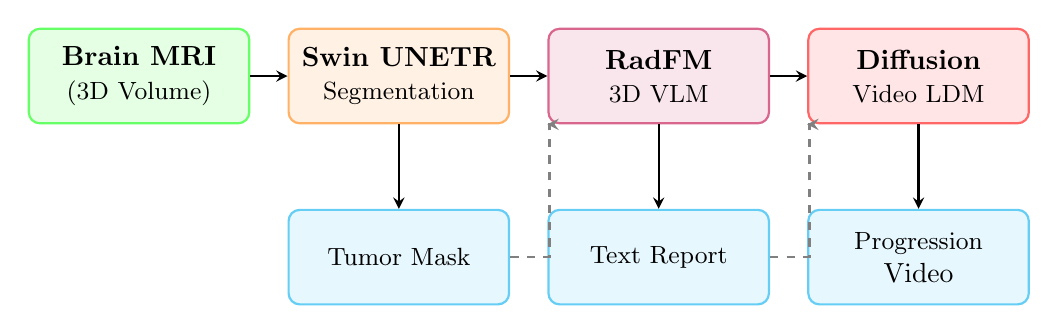
\begin{tikzpicture}[
            node distance=1.8cm,
            box/.style={rectangle, draw=blue!60, fill=blue!10, thick, minimum height=1.2cm, minimum width=2.8cm, align=center, rounded corners},
            arrow/.style={->, thick, >=stealth}
        ]
        
        % Input
        \node[box, fill=green!10, draw=green!60] (input) {\textbf{Brain MRI}\\\small(3D Volume)};
        
        % ViT Segmentation
        \node[box, fill=orange!10, draw=orange!60, right of=input, xshift=1.5cm] (vit) {\textbf{Swin UNETR}\\\small Segmentation};
        
        % LLM
        \node[box, fill=purple!10, draw=purple!60, right of=vit, xshift=1.5cm] (llm) {\textbf{RadFM}\\\small 3D VLM};
        
        % Diffusion
        \node[box, fill=red!10, draw=red!60, right of=llm, xshift=1.5cm] (diff) {\textbf{Diffusion}\\\small Video LDM};
        
        % Outputs
        \node[box, fill=cyan!10, draw=cyan!60, below of=vit, yshift=-0.5cm] (seg) {\small Tumor Mask};
        \node[box, fill=cyan!10, draw=cyan!60, below of=llm, yshift=-0.5cm] (text) {\small Text Report};
        \node[box, fill=cyan!10, draw=cyan!60, below of=diff, yshift=-0.5cm] (video) {\small Progression\\Video};
        
        % Arrows
        \draw[arrow] (input) -- (vit);
        \draw[arrow] (vit) -- (llm);
        \draw[arrow] (llm) -- (diff);
        \draw[arrow] (vit) -- (seg);
        \draw[arrow] (llm) -- (text);
        \draw[arrow] (diff) -- (video);
        
        % Side connections
        \draw[arrow, dashed, gray] (seg.east) -- ++(0.5,0) |- (llm.south west);
        \draw[arrow, dashed, gray] (text.east) -- ++(0.5,0) |- (diff.south west);
        
        \end{tikzpicture}
    \end{center}
    
    \vspace{0.5em}
    
    \begin{columns}
        \begin{column}{0.32\textwidth}
            \centering
            \textbf{Step 1:} Segment\\
            \small Identify tumor regions
        \end{column}
        \begin{column}{0.32\textwidth}
            \centering
            \textbf{Step 2:} Explain\\
            \small Generate text report
        \end{column}
        \begin{column}{0.32\textwidth}
            \centering
            \textbf{Step 3:} Visualize\\
            \small Create progression video
        \end{column}
    \end{columns}
\end{frame}

% ============================================================================
% SLIDE 14: Our Architecture
% ============================================================================
\begin{frame}{Proposed Architecture}
    \begin{columns}
        \begin{column}{0.55\textwidth}
            \begin{block}{Three-Stage Pipeline}
                \small
                \textbf{Stage 1: Segmentation (Swin UNETR)}
                \begin{itemize}\setlength{\itemsep}{0pt}
                    \item Input: Multi-modal MRI (T1, T1c, T2, FLAIR)
                    \item Output: Tumor mask + features
                \end{itemize}
                
                \textbf{Stage 2: Explanation (RadFM)}
                \begin{itemize}\setlength{\itemsep}{0pt}
                    \item Features $\to$ adapter $\to$ text tokens
                    \item RadFM generates report (3D support)
                \end{itemize}
                
                \textbf{Stage 3: Video Generation}
                \begin{itemize}\setlength{\itemsep}{0pt}
                    \item Scan + tokens, time-conditioned
                    \item Video LDM progression frames
                \end{itemize}
            \end{block}
        \end{column}
        
        \begin{column}{0.42\textwidth}
            \begin{block}{Design Choices}
                \small
                \begin{enumerate}\setlength{\itemsep}{2pt}
                    \item \textbf{Modular:} Train separately
                    \item \textbf{Pretrained:} Leverage weights
                    \item \textbf{Interpretable:} Text intermediate
                    \item \textbf{Controllable:} Counterfactual
                \end{enumerate}
            \end{block}
            
            \begin{alertblock}{Novel Contribution}
                \small First system combining all three for tumor progression
            \end{alertblock}
        \end{column}
    \end{columns}
\end{frame}

% ============================================================================
% SLIDE 16: Available Resources Summary
% ============================================================================
\begin{frame}{Available Open-Source Resources}
    \begin{columns}
        \begin{column}{0.48\textwidth}
            \begin{block}{\textcolor{green}{\faIcon{check}} Ready to Use}
                \small
                \textbf{Segmentation:}
                \begin{itemize}\setlength{\itemsep}{0pt}
                    \item \href{https://github.com/Project-MONAI/MONAI}{Swin UNETR} (MONAI)
                    \item \href{https://github.com/MIC-DKFZ/nnUNet}{nnU-Net}
                    \item \href{https://github.com/bowang-lab/MedSAM}{MedSAM}
                \end{itemize}
                
                \textbf{LLMs:}
                \begin{itemize}\setlength{\itemsep}{0pt}
                    \item \href{https://huggingface.co/dmis-lab/biobert-v1.1}{BioBERT}
                    \item \href{https://github.com/microsoft/LLaVA-Med}{LLaVA-Med}
                    \item \href{https://github.com/chaoyi-wu/RadFM}{RadFM}
                \end{itemize}
                
                \textbf{Diffusion:}
                \begin{itemize}\setlength{\itemsep}{0pt}
                    \item \href{https://github.com/CompVis/stable-diffusion}{Stable Diffusion}
                    \item \href{https://arxiv.org/abs/2407.15270}{MedEdit} (paper only)
                \end{itemize}
            \end{block}
        \end{column}
        
        \begin{column}{0.48\textwidth}
            \begin{block}{\textcolor{orange}{\faIcon{exclamation-triangle}} Needs Adaptation}
                \small
                \begin{itemize}\setlength{\itemsep}{1pt}
                    \item Video LDM: No medical weights
                    \item MVG: Not for brain tumors
                \end{itemize}
            \end{block}
            
            
            \begin{exampleblock}{\faIcon{github} Key Repos}
                \scriptsize
                \href{https://github.com/MIC-DKFZ/nnUNet}{MIC-DKFZ/nnUNet}\\
                \href{https://github.com/microsoft/LLaVA-Med}{microsoft/LLaVA-Med}\\
                \href{https://github.com/CompVis/stable-diffusion}{CompVis/stable-diffusion}
            \end{exampleblock}
        \end{column}
    \end{columns}
\end{frame}

% ============================================================================
% SLIDE 15: Available Datasets Overview
% ============================================================================
\begin{frame}{Available Datasets Overview}
    \begin{columns}
        \begin{column}{0.48\textwidth}
            \begin{block}{\href{https://www.synapse.org/brats}{BraTS Challenge}}
                \small
                \begin{itemize}\setlength{\itemsep}{1pt}
                    \item 2,000+ multi-modal MRI volumes
                    \item T1, T1c, T2, FLAIR modalities
                    \item Expert segmentation labels
                \end{itemize}
            \end{block}
            
            \begin{block}{\href{https://physionet.org/content/mimiciii/}{MIMIC-III}}
                \small
                \begin{itemize}\setlength{\itemsep}{1pt}
                    \item 40,000+ ICU patients
                    \item Clinical notes for LLM training
                    \item Free for research
                \end{itemize}
            \end{block}
        \end{column}
        
        \begin{column}{0.48\textwidth}
            \begin{block}{Supporting Datasets}
                \small
                \textbf{\href{https://portal.gdc.cancer.gov/}{TCGA}:} 33 cancer types, multi-modal
                
                \vspace{0.2em}
                
                \textbf{\href{https://wiki.cancerimagingarchive.net/display/Public/LIDC-IDRI}{LIDC-IDRI}:} 1,018 CT scans, multi-annotator
            \end{block}
            
            % \begin{alertblock}{Note}
            %     \small Limited public progression sequences $\Rightarrow$ synthetic augmentation may be needed
            % \end{alertblock}
        \end{column}
    \end{columns}
\end{frame}

% ============================================================================
% SLIDE 16: Conclusion
% ============================================================================
\begin{frame}{Conclusion \& Research Gap}
    \begin{block}{Summary}
        \small
        \begin{itemize}\setlength{\itemsep}{1pt}
            \item \textbf{Problem:} Medical AI lacks explainability + future visualization
            \item \textbf{Solution:} ViT + LLM + Diffusion unified pipeline
            \item \textbf{Innovation:} First explainable tumor progression system
            \item \textbf{Feasibility:} Building on open-source components
        \end{itemize}
    \end{block}
    
    \begin{alertblock}{Research Gap Statement}
        \small
        Current medical AI can segment tumors and generate reports, but \textbf{no existing system simultaneously provides an explanation \textit{and} a ``future'' video of disease progression}. Our project fills this gap by integrating ViT + LLM + diffusion into one pipeline---creating an explainable progression simulator.
    \end{alertblock}
    
    \vspace{0.3em}
    
    \centering
    \Large \textbf{Thank You! Questions?}
\end{frame}

% ============================================================================
% SLIDE 17: References
% ============================================================================
\begin{frame}[allowframebreaks]{Key References}
    \scriptsize
    \begin{thebibliography}{99}
        \bibitem{vit} Dosovitskiy et al., ``\href{https://arxiv.org/abs/2010.11929}{An Image is Worth 16×16 Words},'' ICLR 2021
        \bibitem{swin} Liu et al., ``\href{https://arxiv.org/abs/2103.14030}{Swin Transformer},'' ICCV 2021
        \bibitem{unetr} Hatamizadeh et al., ``\href{https://arxiv.org/abs/2103.10504}{UNETR},'' WACV 2022
        \bibitem{swinunetr} Tang et al., ``\href{https://arxiv.org/abs/2201.01266}{Swin UNETR},'' CVPR 2022
        \bibitem{biobert} Lee et al., ``\href{https://arxiv.org/abs/1901.08746}{BioBERT},'' Bioinformatics 2020
        \bibitem{llavamed} Li et al., ``\href{https://arxiv.org/abs/2306.00890}{LLaVA-Med},'' NeurIPS 2023
        \bibitem{radfm} Wu et al., ``\href{https://arxiv.org/abs/2308.02463}{RadFM},'' arXiv 2023
        \bibitem{ddpm} Ho et al., ``\href{https://arxiv.org/abs/2006.11239}{DDPM},'' NeurIPS 2020
        \bibitem{ldm} Rombach et al., ``\href{https://arxiv.org/abs/2112.10752}{Latent Diffusion},'' CVPR 2022
        \bibitem{videoldm} Blattmann et al., ``\href{https://arxiv.org/abs/2304.08818}{Video LDM},'' ICCV 2023
        \bibitem{mvg} Cao et al., ``\href{https://openaccess.thecvf.com/content/CVPR2024/html/Cao_MVG_CVPR_2024_paper.html}{MVG},'' CVPR 2024
        \bibitem{medeidt} Ben Alaya et al., ``\href{https://arxiv.org/abs/2407.15270}{MedEdit},'' MICCAI 2024
        \bibitem{medsam} Ma et al., ``\href{https://www.nature.com/articles/s41467-024-44824-z}{MedSAM},'' Nature Communications 2024
    \end{thebibliography}
\end{frame}

\end{document}
